\documentclass[12pt,fontset=none]{ctexbook}

%导入宏包
\usepackage{amsmath,amssymb}
\usepackage{xcolor}
\usepackage{fancyhdr,fancybox}
\usepackage{geometry}
\usepackage[hidelinks]{hyperref}
\usepackage[many,most]{tcolorbox}
\usepackage{tkz-euclide}
%\usepackage{mathptmx} 


%字体设置
\usepackage {xeCJK}                                     
\setCJKmainfont {KaiTi}
%Arial Unicode MS
%FangSong,仿宋
%KaiTi,楷体
%Microsoft YaHei,微软雅黑
%MingLiU,细明体
%NSimSun,新宋体
%PMingLiU,新细明体
%SimHei,黑体
%SimSun,宋体


%页面设置
\geometry{a4paper,left=2cm,right=2cm,top=2cm,bottom=2.5cm}

%页眉页码
\pagestyle{fancy}
\fancyhf{}
\chead{\leftmark}
%\lhead{Guides and tutorials}
\cfoot{\thepage}
%\fancyhead[LE,RO]{\thepage}
%\fancyhead[CE,CO]{\leftmark}
%\fancyfoot[CE,CO]{\leftmark}
%\fancyfoot[LE,RO]{\thepage}
\renewcommand{\headrulewidth}{2pt}
%\renewcommand{\footrulewidth}{1pt}



%定义命令
\newcommand{\ndef}{\noindent\textbf{定义:} }

%定义环境
%\renewenvironment{deg}[1][]{\rm{deg\,}}{\par}
\newenvironment{proof}[1][]{\par \noindent \textbf{\hspace{2em}证明 \vspace{0.1mm} #1 :}}{\par}
%定义复数i
\renewcommand{\i}{\mathrm{i}}
%定义e
\newcommand{\e}{\mathrm{e}}
%定义共轭符号
\newcommand{\Lin}[1]{\overline{#1}}
%定义直体
\renewcommand{\rm}[1]{\mathrm{#1}\,}

%例
\newcounter{example}
\counterwithin*{example}{section}
\newenvironment{example}[1][]{%
\stepcounter{example}%
\par\vspace{5pt}\noindent
\fbox{\textbf{例:~\thesection.\theexample}}%
\hrulefill\par\vspace{10pt}\noindent\rmfamily}%
{\par\noindent\hrulefill\vrule width10pt height2pt depth2pt\par}
%示例
\newcounter{instance}
\counterwithin*{instance}{section}
\newenvironment{instance}[1][]{%
\stepcounter{instance}%
\par\vspace{5pt}\noindent
\fbox{\textbf{示例:~\thesection.\theexample}}%
\hrulefill\par\vspace{10pt}\noindent\rmfamily}%
{\par\noindent\hrulefill\vrule width10pt height2pt depth2pt\par}
%问题
\newcounter{problem}
\counterwithin*{problem}{section}
\newenvironment{problem}[1][]{%
\stepcounter{problem}%
\par\vspace{5pt}\noindent
\fbox{\textbf{问题:~\thesection.\theexample}}%
\hrulefill\par\vspace{10pt}\noindent\rmfamily}%
{\par\noindent\hrulefill\vrule width10pt height2pt depth2pt\par}
%练习
\newcounter{exercise}
\counterwithin*{exercise}{section}
\newenvironment{exercise}[1][]{%
\stepcounter{exercise}%
\par\vspace{5pt}\noindent
\fbox{\textbf{练习:~\thesection.\theexample}}%
\hrulefill\par\vspace{10pt}\noindent\rmfamily}%
{\par\noindent\hrulefill\vrule width10pt height2pt depth2pt\par}

\newenvironment{remark}[1][]{\par \noindent \textbf{\hspace{2em}注 \vspace{0.1mm} :}}{\par}
\newenvironment{assumption}[1][]{\par \noindent \textbf{假设 \vspace{0.1mm}  :}}{\par}
%结论
\newcounter{conclusion}
\counterwithin*{conclusion}{section}
\newenvironment{conclusion}[1][]{%
\stepcounter{conclusion}%
\par\vspace{5pt}\noindent
\fbox{\textbf{结论:~\thesection.\theexample}}%
\hrulefill\par\vspace{10pt}\noindent\rmfamily}%
{\par\noindent\hrulefill\vrule width10pt height2pt depth2pt\par}

\newenvironment{solution}[1][]{\par \noindent \textbf{解 \vspace{0.1mm}  :}}{\par}
%性质
\newcounter{property}
\counterwithin*{property}{section}
\newenvironment{property}[1][]{%
\stepcounter{property}%
\par\vspace{5pt}\noindent
\fbox{\textbf{性质:~\thesection.\theexample}}%
\hrulefill\par\vspace{10pt}\noindent\rmfamily}%
{\par\noindent\hrulefill\vrule width10pt height2pt depth2pt\par}


\newtcolorbox{bdef}[1]{%定理,公理,公设,引理,命题,推论
  breakable,enhanced,enlarge top by=0mm,colback=white,colframe=black,fonttitle=\bfseries,colbacktitle=white,coltitle=black,attach boxed title to top left={xshift=3mm,yshift*=-\tcboxedtitleheight/2},title=#1,boxrule=1.0pt}
\setlength{\headheight}{27pt}

%封面
\title{\fontsize{42pt}{\baselineskip}\selectfont 复变函数---习题解答}

\date{\vspace{16cm}\fontsize{21pt}{\baselineskip}\selectfont \today}

\begin{document}
\maketitle
\everymath{\displaystyle}
\thispagestyle{empty}
\tableofcontents
\setcounter{page}{0}
\thispagestyle{empty}
\newpage
%正文区

\chapter{复数与复变函数}
\newpage
\section{复数的定义及其运算}
1.设$z$和$w$是两个复数,证明:
\begin{enumerate}
  \item[(1)] $\rm{Re} z =\frac{1}{2}(z + \overline{z}),\;\rm{Im} z =\frac{1}{2i}(z-\overline z);$
  \item[(2)] $z\overline{z}=|z|^{2};$
  \item[(3)] $\overline{z+w}=\overline{z}+\overline{w},\; \overline{zw}=\overline{z}\overline{w};$
  \item[(4)] $|zw|=|z||w|,\,\left|\frac{z}{w}\right|=\frac{|z|}{|w|};$
  \item[(5)] $|z|=|\overline{z}|.$
\end{enumerate}
\begin{proof}
    设$z=a+b\i,w=u+v\i$,则
    \begin{enumerate}
      \item [(1)] $\rm{Re}z =a =\frac{1}{2}[(a+b\i)+(a-b\i)]=\frac{1}{2}(z+\overline{z});$
      \item [(2)] $z\Lin{z}=(a+b\i)(a-b\i)=a^{2}+b^{2}=|z|^{2};$
      \item [(3)] $\Lin{z+w}=\Lin{(a+b\i)+(u+v\i)}=\Lin{(a+u)+(b+v)\i}=(a+u)-(b+v)\i=(a-b\i)+(u-v\i)=\Lin{z}+\Lin{w}; $
      \item [(4)] $|zw|^{2}=(zw)\Lin{(zw)}=|z|^{2}|w|^{2}$,两边同时开方即得(4);
      \item [(5)] $|z|=\sqrt{a^{2}+b^{2}}=\sqrt{a^{2}+(-b)^{2}}=|\Lin{z}|^{2}.$
    \end{enumerate}
\end{proof}

\

2.设$z_{1},\cdots,z_{n}$是任意$n$个复数,证明:
$$|z_{1}+z_{2}+\cdots+z_{n}| \leqslant |z_{1}|+|z_{2}|+\cdots+|z_{n}|,$$
并给出不等式中等号成立的条件.
\begin{proof}
  由复数模的三角不等式可得$|z_{1}+z_{2}+\cdots+z_{n}| \leqslant |z_{1}+z_{2}+\cdots+z_{n-1}|+|z_{n}|$,等号成立当且仅当存在$t_{n} \geqslant 0$使得$z_{1}+z_{2}+\cdots+z_{n-1}=t_{n}z_{n}$,继续对不等式右侧第一项的$n-1$个复数使用复数模的三角不等式可得
  $$|z_{1}+z_{2}+\cdots+z_{n}| \leqslant |z_{1}+z_{2}+\cdots+z_{n-1}|+|z_{n}| \leqslant |z_{1}+z_{2}+\cdots+z_{n-2}|+|z_{n-1}|+|z_{n}|$$
  等号成立当且仅当存在满足上述的$t_{n}$,并且存在$t_{n-1} \geqslant 0$使得$z_{1}+z_{2}+\cdots+z_{n-2}=t_{n-1}z_{n-1}$,于是可得$(t_{n-1}+1)z_{n-1}=t_{n}z_{n}$,即$z_{n-1}$与$z_{n}$共线且同向,如此递归地进行$n-1$次可得
  $$|z_{1}+z_{2}+\cdots+z_{n}| \leqslant |z_{1}|+|z_{2}|+\cdots+|z_{n}|,$$
  等号成立当且仅当存在$n$个非负实数$k_{1},\cdots.k_{n}$,使得
  $$k_{1}z_{1}=k_{2}z_{2}=\cdots=k_{n}z_{n}.$$
\end{proof}

\

3.证明:
$$\frac{1}{\sqrt{2}}(|\rm{Re}z|+|\rm{Im}z|) \leqslant |z| \leqslant |\rm{Re}z|+|\rm{Im} z|.$$
\begin{proof}
    设$z=a+b\i$,则$\rm{Re}z=a,\rm{Im}z=b,|z|=\sqrt{a^{2}+b^{2}}$,即证
    $$\frac{1}{\sqrt{2}}(|a|+|b|) \leqslant \sqrt{a^{2}+b^{2}}\leqslant |a|+|b|,$$
    等价于证
    $$\frac{1}{2}(|a|+|b|)^{2} \leqslant a^{2}+b^{2} \leqslant (|a|+|b|)^{2},$$
    对左边不等式,由$(|a|-|b|)^{2} \geqslant 0$,可得$2|a||b| \leqslant |a|^{2}+|b^{2}|$,两边同时加$ |a|^{2}+|b^{2}|$再除以2即得$\frac{1}{2}(|a|+|b|)^{2} \leqslant a^{2}+b^{2} $;对右边不等式,由$a^{2}+b^{2} \leqslant |a|^{2}+2|a||b|+|b|^{2}$,显然可得,$a^{2}+b^{2} \leqslant (|a|+|b|)^{2}$
\end{proof}

\

4.若$|z_{1}|=\lambda|z_{2}|,\lambda > 0$,证明:
$$|z_{1} - \lambda^{2}z_{2}|=\lambda|z_{1}-z_{2}|.$$
\begin{proof}
    $$
    \begin{aligned}
      |z_{1}-\lambda^{2}z_{2}|^{2}= (z_{1}-\lambda^{2}z_{2})(\Lin{z_{1}}-\lambda^{2}\Lin{z_{2}}) = & |z_{1}|^{2}-\lambda^{2}z_{2}\Lin{z_{1}}-\lambda^{2}z_{1}\Lin{z_{2}}+\lambda^{4}|z_{2}|^{2}\\
      = & \lambda^{2}|z_{2}|^{2}-\lambda^{2}z_{2}\Lin{z_{1}}-\lambda^{2}z_{1}\Lin{z_{2}}+\lambda^{2}|z_{1}|^{2} \\
      = & \lambda^{2}(|z_{2}|^{2}-z_{2}\Lin{z_{1}}-z_{1}\Lin{z_{2}}+|z_{1}|^{2}) \\
      = & \lambda^{2}(z_{1}-z_{2})\Lin{(z_{1}-z_{2})} \\
      = & \lambda^{2}|z_{1}-z_{2}|^{2}.
    \end{aligned}
    $$
    同时开方即得
    $$|z_{1} - \lambda^{2}z_{2}|=\lambda|z_{1}-z_{2}|.$$
\end{proof}

\

5.设$|a| <1 $,证明:若$|z|=1$,则
$$\left|\frac{z-a}{1-\Lin{a}z}\right|=1.$$
\begin{proof}
    $|1-\Lin{a}z|=|z|\left|\frac{1}{z}-\Lin{a}\right|=|\Lin{z}-\Lin{a}|=|\Lin{z-a}|=|z-a|.$
\end{proof}

\

6.设$|a| < 1,|z| <1$.证明:
\begin{enumerate}
  \item[(1)] $\left|\frac{z-a}{1-\Lin{a}z}\right| < 1$;
  \item[(2)] $1-\left|\frac{z-a}{1-\Lin{a}z}\right|^{2}=\frac{(1-|a|^{2})(1-|z|^{2})}{|1-\Lin{a}z|^{2}}$;
  \item[(3)] $\frac{||z|-|a||}{1-|a||z|} \leqslant \left|\frac{z-a}{1-\Lin{a}z}\right| \leqslant \frac{|z|+|a|}{1+|a||z|}$.   
\end{enumerate}
\begin{proof}
    %注意到(1),(2),(3)在变换$z \to z\e^{\i \theta},\,a \to a \e^{\i \theta}$下不变,故不妨设$a \in \mathbb{R}$.
    \begin{enumerate}
      \item[(1)] 由于
      $$|z-a|^{2}=(z-a)\Lin{(z-a)}=(z-a)(\Lin{z}-\Lin{a})=|z|^{2}+|a|^{2}-a\Lin{z}-\Lin{a}z,$$
      $$|1-\Lin{a}z|^{2}=(1-\Lin{a}z)\Lin{(1-\Lin{a}z)}=(1-\Lin{a}z)(1-a\Lin{z})=1+|a|^{2}|z|^{2}-a\Lin{z}-\Lin{a}z,$$
      故原命题等价于证:
      $$|z|^{2}+|a|^{2} < 1+|a|^{2}|z|^{2} $$
      其中$|z|<1,|a|<1$.由$(1-|z|^{2})(1-|a|^{2})=1-|z|^{2}-|a|^{2}+|a|^{2}|z|^{2} > 0$,从而命题得证.
      \item[(2)] 原命题等价于证:
      $$|1-\Lin{a}z|^{2}-|z-a|^{2}=(1-|a|^{2})(1-|z|^{2}),$$
      由(1)可知
      $$|1-\Lin{a}z|^{2}-|z-a|^{2}=1+|a|^{2}|z|^{2}-|z|^{2}-|a|^{2}=(1-|a|^{2})(1-|z|^{2})$$
      \item[(3)] $$1-\left[\frac{||z|-|a||}{1-|a||z|}\right]^{2}=\frac{(1-|a|^{2})(1-|z|^{2})}{(1-|a||z|)^{2}},$$
      $$1-\left[\frac{|z|+|a|}{1+|a||z|}\right]^{2}=\frac{(1-|a|^{2})(1-|z|^{2})}{(1+|a||z|)^{2}},$$
      由复数模的三角不等式显然可得$1-|a||z| \leqslant |1-\Lin{a}z| \leqslant 1+|a||z|$,从而
      $$\frac{(1-|a|^{2})(1-|z|^{2})}{(1+|a||z|)^{2}} \leqslant \frac{(1-|a|^{2})(1-|z|^{2})}{|1-\Lin{a}z|^{2}} \leqslant   \frac{(1-|a|^{2})(1-|z|^{2})}{(1-|a||z|)^{2}},$$ 
      于是由(2)可得
      $$1-\left[\frac{|z|+|a|}{1+|a||z|}\right]^{2} \leqslant 1-\left|\frac{z-a}{1-\Lin{a}z}\right|^{2} \leqslant 1-\left[\frac{||z|-|a||}{1-|a||z|}\right]^{2}.$$
      即
      $$\frac{||z|-|a||}{1-|a||z|} \leqslant \left|\frac{z-a}{1-\Lin{a}z}\right| \leqslant \frac{|z|+|a|}{1+|a||z|}.$$
    \end{enumerate}
\end{proof}

\

7.设$z_{1},\cdots,z_{n},w_{1},\cdots,w_{n}$是任意$2n$个复数,证明复数形式的Lagrange等式:
$$\big|\sum\limits_{j=1}^{n}z_{j}w_{j}\big|^{2}=(\sum\limits_{j=1}^{n}|z_{j}|^{2})(\sum\limits_{j=1}^{n}|w_{j}|^{2})-\sum\limits_{1 \leqslant j <k \leqslant n}|z_{j}\Lin{w_{k}}-z_{k}\Lin{w_{j}}|^{2},$$
并由此推出Cauchy不等式:
$$\big|\sum\limits_{j=1}^{n}z_{j}w_{j}\big|^{2} \leqslant (\sum\limits_{j=1}^{n}|z_{j}|^{2})(\sum\limits_{j=1}^{n}|w_{j}|^{2}),$$
不等式中等号成立的条件是什么?
\begin{proof}
    $$
    \begin{aligned}
      \big|\sum\limits_{j=1}^{n}z_{j}w_{j}\big|^{2}-(\sum\limits_{j=1}^{n}|z_{j}|^{2})(\sum\limits_{j=1}^{n}|w_{j}|^{2})= &
      \left|\begin{matrix}
        \sum\limits_{j=1}^{n}z_{j}w_{j} & \sum\limits_{j=1}^{n}|z_{j}|^{2} \\
        \sum\limits_{j=1}^{n}|w_{j}|^{2} & \sum\limits_{j=1}^{n}\Lin{z_{j}w_{j}} \\
      \end{matrix}\right| \\
      =&
      \left|
          \begin{pmatrix}
            z_{1} & z_{2} & \cdots & z_{n} \\
            \Lin{w_{1}} & \Lin{w_{2}} & \cdots & \Lin{w_{n}} \\ 
          \end{pmatrix}
          \begin{pmatrix}
            w_{1} & \Lin{z_{1}} \\
            w_{2} & \Lin{z_{2}} \\
            \vdots & \vdots \\
            w_{n} & \Lin{z_{n}} \\
          \end{pmatrix}
        \right| \\
        = & \sum\limits_{1 \leqslant j < k \leqslant n} 
        \left|\begin{matrix}
            z_{j} & z_{k} \\
            \Lin{w_{j}} & \Lin{w_{k}}
        \end{matrix}\right|
        \left|\begin{matrix}
          w_{j} & \Lin{z_{j}} \\
          w_{k} & \Lin{z_{k}}
      \end{matrix}\right| \quad (\rm{Cauchy-Binet}\text{公式})\\
      =&-\sum\limits_{1 \leqslant j < k \leqslant n}|z_{j}\Lin{w_{k}}-z_{k}\Lin{w_{j}}|^{2}.
    \end{aligned}
    $$
    由复数模的非负性显然可得Cauchy不等式:
    $$\big|\sum\limits_{j=1}^{n}z_{j}w_{j}\big|^{2} \leqslant (\sum\limits_{j=1}^{n}|z_{j}|^{2})(\sum\limits_{j=1}^{n}|w_{j}|^{2}),$$
    等号成立当且仅当对任意$1 \leqslant j < k \leqslant n$,都有$z_{j}\Lin{w_{k}}=z_{k}\Lin{w_{j}}$,即存在复常数$k$,使得$(z_{j},z_{k})=k(\Lin{w_{j}},\Lin{w_{k}})$,由任意性可得,等号成立当且仅当即存在复常数$k$使得
    $$(z_{1},z_{2},\cdots,z_{n})=k(\Lin{w_{1}},\Lin{w_{2}},\cdots,\Lin{w_{n}}).$$
\end{proof}

\

8.设$z_{1},\cdots,z_{n}$是任意$n$个复数,证明必有$\{1,2,\cdots,n\}$的子集$E$,使得
$$\big|\sum\limits_{j \in E} z_{j}\big| \geqslant \frac{1}{6}\sum\limits_{j=1}^{n} |z_{j}| .$$
\begin{proof}
    将复平面按象限分成四个闭集,则这四个闭集中至少有一个闭集记作$A$,使得
    $$\sum\limits_{z_{j} \in A}|z_{j}| \geqslant \frac{1}{4}\sum\limits_{j=1}^{n}|z_{j}|,$$
    由于同一象限中复数的实部与虚部的符号相同,不妨设$A$为第一象限与其边界组成的闭集,则对任一$z \in A$,记$z=|z|\e^{{\i \theta}},\, \theta \in [0,\frac{\pi}{2}]$,则$z$在$\theta=\frac{\pi}{4}$上的投影为$|z|\e^{\i \frac{\pi}{4}}\cos(\frac{\pi}{4}-\theta)$,并且易得
    $$\big||z|\e^{\i \frac{\pi}{4}}\cos(\frac{\pi}{4}-\theta)\big| \geqslant \frac{\sqrt{2}}{2}|z|,$$
    记$z_{j} \in A$的指标集为$E$,则
    $$
    \begin{aligned}
      \big|\sum\limits_{j \in E} z_{j}\big|\geqslant \big|\sum\limits_{j \in E} |z_{j}|\e^{\i \frac{\pi}{4}}\cos(\frac{\pi}{4}-\theta_{j})\big|= & \sum\limits_{j \in E}\big||z_{j}|\e^{\i \frac{\pi}{4}}\cos(\frac{\pi}{4}-\theta_{j})\big| \\
      \geqslant & \frac{\sqrt{2}}{2}\sum\limits_{j \in E}|z_{j}| 
      \geqslant  \frac{\sqrt{2}}{8}\sum\limits_{j =1}^{n}|z_{j}| 
      \geqslant  \frac{1}{6}\sum\limits_{j =1}^{n}|z_{j}|.
    \end{aligned}
    $$
   
\end{proof}

\begin{remark}
    在分割闭集时可以按$y=\pm x$分割,这样讨论更方便.更一般的可以将系数改进到$\frac{1}{\pi}$.(详见Rudin实分析与复分析\; 6.3)
\end{remark}




\newpage
\section{复数的几何表示}
1.把复数$z=1+\cos \theta + \i \sin \theta$写成三角形式.


2.问$n$取何值时有$(1+\i)^{n}=(1-\i)^{n}$?


3.证明:
$$\sum\limits_{k=0}^{n}\cos k\theta=\frac{\sin \frac{\theta}{2}+\sin\left(n+\frac{1}{2}\right)\theta}{2\sin \frac{\theta}{2}},\;\sum\limits_{k=1}^{n}\sin k\theta=\frac{\cos \frac{\theta}{2}-\cos\left(n+\frac{1}{2}\right)\theta}{2\sin \frac{\theta}{2}}.$$

4.证明:$\bigtriangleup z_{1}z_{2}z_{3}$和$\bigtriangleup w_{1}w_{2}w_{3}$同向相似的充分必要条件为
$$
\begin{vmatrix}
  z_{1} & w_{1} & 1 \\
  z_{2} & w_{2} & 1 \\
  z_{3} & w_{3} & 1 \\
\end{vmatrix}=0.
$$


5.设$z_{1}\neq z_{2}$,证明:
\begin{enumerate}
  \item [(1)] $z$位于以$z_{1}$和$z_{2}$为端点的开线段上,当且仅当存在$\lambda \in (0,1)$,使得
  $$z=\lambda z_{1}+(1-\lambda)z_{2};$$
  \item[(2)] $z$位于以$z_{1}$和$z_{2}$为端点的开圆弧上,当且仅当存在$\theta\,(0<|\theta|<\pi)$,使得
  $$\arg \frac{z-z_{1}}{z-z_{2}}=\theta.$$
\end{enumerate}

6.证明:三点$z_{1},z_{2},z_{3}$共线的充要条件为
$$
\begin{vmatrix}
  z_{1} & \Lin{z_{1}} & 1 \\
  z_{2} & \Lin{z_{2}} & 1 \\
  z_{3} & \Lin{z_{3}} & 1 \\
\end{vmatrix}=0.
$$

7.下图是三个边长为$1$的正方形    
\begin{center}
  \begin{tikzpicture}[thick, scale = 1.5]
    \draw (0,0) node[below]{$O$} -- (3,0) node[below]{$D$} -- (3,1) node[above]{$C$}
      -- (2,1) node[above]{$B$} -- (1,1) node[above]{$A$} -- (0,1) -- cycle;
    \draw (0,0) -- (1,1) (0,0) -- (2,1) (0,0) -- (3,1);
    \draw (1,0) -- (1,1) (2,0) -- (2,1);
  \end{tikzpicture}
\end{center}
\quad\quad 证明:
$$\angle AOD+ \angle BOD +\angle COD =\frac{\pi}{2}.$$

8.如图,$ABED,ACFG$是正方形,$AH\bot BC$,$M$是$DG$的中点.证明:$M,A,H$三点共线.
\begin{center}
  \begin{tikzpicture}[thick]
    \tkzDefPoints{0/0/B, 2/0/C, 0.8/1.2/A}
    \tkzDefSquare(B,A) \tkzGetPoints{D}{E}
    \tkzDrawPolygon[thick](B,A,D,E)
    \tkzDefSquare(A,C) \tkzGetPoints{F}{G}
    \tkzDrawPolygon[thick](A,C,F,G)
    \tkzDefMidPoint(D,G) \tkzGetPoint{M}
    \tkzInterLL(M,A)(B,C)
    \tkzGetPoint{H}
    \draw (B) -- (C) (D) -- (G)(M) -- (H);
    \tkzMarkRightAngle[scale=0.5](C,H,M)
    \tkzLabelPoints[below](B,C,H)
    \tkzLabelPoints[above](D,M,G)
    \tkzLabelPoints[right](A,F)
    \tkzLabelPoints[left](E)
  \end{tikzpicture}
\end{center}
    


9.如图,在平行四边形$ABCD$中,如果
$$\Lin{AC}^{2} \cdot \Lin{BD}^{2}=\Lin{AB}^{4}+\Lin{AD}^{4},$$
那么这个平行四边形的锐角等于$\frac{\pi}{4}$.
\begin{center}
  \begin{tikzpicture}[thick]
    \draw (0,0) coordinate(A) node[below]{$A$} -- ++(4,0) coordinate(B) node[below]{$B$}
    -- ++ (2,2) coordinate(C) node[above]{$C$} -- ++(-4,0) coordinate(D) node[above]{$D$}
    --cycle;
    \draw (A) -- (C) (B) -- (D);
  \end{tikzpicture}
\end{center} 


10.证明:
$$|z_{1}+z_{2}|^{2}+|z_{1}-z_{2}|^{2}=2(|z_{1}|^{2}+|z_{2}|^{2}),$$
并说明等式的几何意义.

11.设$z_{1},\cdots,z_{n}$是单位圆周(以原点为中心、半径为$1$的圆周)上的$n$个点,如果$z_{1},\cdots,z_{n}$是正$n$边形的$n$个顶点,证明:
$$z_{1}+z_{2}+\cdots+z_{n}=0.$$

12.设$z_{1},z_{2},z_{3}$是单位圆周上的三个点,证明:这三个点是一正三角形三个顶点的充要条件为
$$z_{1}+z_{2}+z_{3}=0.$$

13.设$z_{1},z_{2},z_{3},z_{4}$是单位圆周上的四个点,证明:这四个点是一矩形顶点的充要条件为
$$z_{1}+z_{2}+z_{3}+z_{4}=0.$$


14.设$L$是由方程
$$az\Lin{z}+\Lin{\beta}z+\beta \Lin{z} +d=0,$$
所确定的点的轨迹,其中$a,d$是实数,$\beta$是复数.证明:
\begin{enumerate}
  \item[(1)] 当$a=0,\, \beta \neq 0$时,$L$是一直线;
  \item[(2)] 当$a \neq 0,|\beta|^{2}-ad > 0$时,$L$是一圆周,并求出该圆周的圆心和半径.  
\end{enumerate}


15.设$z_{1}\neq z_{2},0< \lambda \neq 1$,证明由方程
$$\left|\frac{z-z_{1}}{z-z_{2}}\right|=\lambda,$$
所确定的点$z$的轨迹是一圆周(通常称为Apollonius圆),该圆周的圆心$a$和半径$R$分别为
$$a=\frac{z_{1}-\lambda^{2}z_{2}}{1-\lambda^{2}},\quad R=\frac{\lambda|z_{1}-z_{2}|}{|1-\lambda^{2}|}.$$


16.如果$z_{1},\cdots,z_{n}$都位于过原点的直线的一侧,证明$\frac{1}{z_{1}},\cdots,\frac{1}{z_{n}}$也必位于该直线的某一侧,而且满足
$$z_{1}+\cdots+z_{n}=0,\quad \frac{1}{z_{1}}+\cdots + \frac{1}{z_{n}}\neq 0.$$


17.设$z_{1},\cdots,z_{n}$是一个凸$n$边形的$n$个顶点,如果$a$满足关系
$$\frac{1}{z_{1}-a}+\cdots+\frac{1}{z_{n}-a}=0,$$
那么$a$必在这个凸$n$边形的内部.


18.证明:
$$\sin \frac{\pi}{n}\sin\frac{2\pi}{n}\cdots\sin\frac{(n-1)\pi}{n}=\frac{n}{2^{n-1}}.$$
(\textbf{提示:}考虑方程式$(z+1)^{n}=1$的$n-1$个不为零的根的乘积.)

19.设$0<\theta < \frac{\pi}{2},\; P_{m}(x)=\sum\limits_{k=0}^{m}(-1)^{k}\binom{2m+1}{2k+1}x^{m-k} $.证明:
$$\sin(2m+1)\theta=\sin^{2m+1}\theta P_{m}(\rm{ctg}^{2}\theta).$$

20.利用上题结果证明:
\begin{enumerate}
  \item[(1)] $\sum\limits_{k=1}^{m} \rm{ctg}^{2}\frac{k\pi}{2m+1}=\frac{m(2m-1)}{3}$;
  \item[(2)] $\prod\limits_{k=1}^{m}\rm{ctg}^{2}\frac{k\pi}{2m+1}=\frac{1}{2m+1}$.  
\end{enumerate}


















\newpage
\section{扩充平面和复数的球面表示}
1.证明:在复数的球面表示下,$z$和$\frac{1}{z}$的球面像关于复平面对称.
\begin{proof}
  
\end{proof}

\

2.证明:在复数的球面表示下,$z$和$w$的球面像是直径对点当且仅当$z\Lin{w}=-1$.
\begin{proof}
  
\end{proof}

\

3.证明:在复数的球面表示下,$\mathbf{C}_{\infty}$中的点$z$和$w$的球面像间的距离为$\frac{2|z-w|}{\sqrt{(|z|^{2}+1)(|w|^{2}+1)}}$.
\begin{proof}
  
\end{proof}

\

4.证明:在复数的球面表示下,若$\begin{pmatrix}
  a & b \\
  c & d \\
\end{pmatrix}$是二阶酉方阵,则$\mathbf{C}_{\infty}$的变换$w=\frac{az+b}{cz+d}$诱导了球面绕球心的一个旋转.
\begin{proof}
  
\end{proof}

\

5.证明:在复数的球面表示下,球面上圆周对应于复平面上的圆周或直线,反之亦然.
\begin{proof}
  
\end{proof}

\

6.证明:在复数的球面表示下,复平面上两条光滑曲线在交点处的夹角与它们的球面像在交点处的夹角相等.
\begin{proof}
  
\end{proof}

\newpage
\section{复数列的极限}
1.设$z_{0} \notin (-\infty,0],\,z_{n} \neq 0,\; \forall\, n \in \mathbf{N} $.证明:复数列$\{z_{n}\}$收敛到$z_{0}$的充要条件是$\lim\limits_{n \to \infty}|z_{n}|=|z_{0}|$和$\lim\limits_{n \to \infty}\arg z_{n}=\arg z_{0}$.
\begin{proof}
  
\end{proof}

\

2.设$z=x+\i y \in \mathbf{C}$,证明:
$$\lim\limits_{nn \to \infty}\left(1+\frac{z}{n}\right)^{z}= \e^{x}(\cos y+ \i \sin y) .$$
\begin{proof}
  
\end{proof}

\

3.证明:若$\lim\limits_{n\to \infty}z_{n}=z_{0}$,则
$$\lim\limits_{n \to \infty }\frac{z_{1}+z_{2}+\cdots+z_{n}}{n}=z_{0}.$$
\begin{proof}
  
\end{proof}

\

4.证明:若$\lim\limits_{n \to \infty}z_{n}=z_{0},\;\lim\limits_{n \to \infty}w_{n}=w_{0}$,则
$$\lim\limits_{n \to \infty}\frac{1}{n}\sum\limits_{k=1}^{n}z_{k}w_{n-k}=z_{0}w_{0}.$$
\begin{proof}
  
\end{proof}

\

5.设无穷三角阵
$$
\begin{matrix}
  a_{11} & & \\
  a_{21} & a_{22} & \\
  a_{31} & a_{32} & a_{33}\\
  \cdots & \cdots & \cdots \\
\end{matrix}
$$
满足\begin{enumerate}
  \item [(1)] 对任意固定的$k$,$\lim\limits_{n \to \infty}a_{nk}=a_{k}$存在;
  \item [(2)] $\lim\limits_{n \to \infty}\sum\limits_{k=1}^{n}a_{nk}$存在;
  \item [(3)] $\sum\limits_{k=1}^{n}|a_{nk}| \leqslant M < \infty,\,\forall \, n \in \mathbf{N}$.
\end{enumerate}
证明:若复数列$\{z_{n}\}$收敛,则$\lim\limits_{n \to \infty}\sum\limits_{k=1}^{n}a_{nk}z_{k}$存在.
\begin{proof}
  
\end{proof}




\newpage
\section{开集、闭集和紧集}
1.证明:一个平面点集的孤立点的全体至多可列.






\newpage
\section{曲线和域}
\newpage
\section{复变函数的极限和连续性}
\newpage


\chapter{全纯函数}
\newpage
\section{复变函数的导数}
\newpage
\section{Cauchy-Riemann方程}
\newpage
\section{导数的几何意义}
\newpage
\section{初等全纯函数}
\newpage
\section{分式线性变换}
\newpage

\chapter{全纯函数与积分表示}
\chapter{全纯函数的Taylor展开及其应用}
\chapter{全纯函数的Laurent展开及其应用}
\chapter{全纯开拓}
\chapter{共形映射}
\chapter{调和函数与次调和函数}
\chapter{多复变全纯函数与全纯映射}

\end{document}